% Chapter 10

\chapter{Correction factors to the multiplicities} % Chapter title

\label{ch:CF} % For referencing the chapter elsewhere, use \autoref{ch:name}

%----------------------------------------------------------------------------------------

The \textit{raw} charged multiplicities presented in the previous chapter need to be corrected. The corrections discussed are acceptance correction ie. the correction due to the geometrical limitation of the spectrometer and the data reconstruction efficiency, diffractive vector meson correction, radiative correction or electron contamination correction.

\section{Determination of the spectrometer acceptance}

\subsection{Monte Carlo sample from DJANGOH}

The COMPASS detector does not cover the full phase-space then the measured multiplicities have
to be corrected for the finite detector acceptance of the order of 70\%. The correction is
done using a Monte-Carlo dataset containing about 400 million events generated in the kinematic
region $Q^2 > 0.8$ (GeV/c)$^2$, $x$ $\in$ [10$^{-4}$,0.9], $y$ $\in$ [0.01,0.95], thanks to the Blue Waters facility computing power \cite{}. The kinematic region is larger than the one of interest in the analysis. This is done in order to be able to take into account smearing effects. These 400 millions events are divided in 4 different samples. As there is a difference in the experimental setup between P07 and P08 onwards (two slabs in the OT), two different acceptance corrections should be applied. On the same basis, it was decided that the different beam charge should also have their own sample as there might be asymmetries in the spectrometer concerning the beam charge.

The events are created with DJANGOH generator with parametrization of the parton distribution functions (MSTW08). In addition, the use of JETSET inside DJANGOH allows the hadronization of quarks q to final-state hadrons h according to the Lund model. The COMPASS high $p_T$ tuning was used. The events of DJANGOH are then propagated into the experimental setup simulated by TGEANT. The output of this chain is referred to as \textit{generated} sample. This events are then reconstructed with the same CORAL that was used to reconstruct real data. This new sample is called \textit{reconstructed} sample. The same DIS event and unidentified hadron selection that are used on real data (except the BMS cut) are applied to the MC data sample for reconstructed MC events and particles.

The acceptance involves both reconstructed and generated particles. In both cases, the particle ID is taken from the MC truth. The following selection is made on the generated events and particles :

\begin{enumerate}
  \item Energy of the beam muon in range [140,180] GeV
	\item Z coordinate of event vertex ($z_{vtx}$) within the target region $\in$ [-325 cm, -71 cm]
	\item Primary interaction in the target material (PHAST routine PaAlgo:InTarget() for both data and MC (Section \ref{Raw}) target positions
				to have a complete overlap of coverage)
	\item Beam track crossing the entire target (PHAST routine PaAlgo:CrossCells())
  \item $Q^2>1$ (GeV/c)$^2$
  \item $0.1 < y < 0.7$
	\item $5 < W < 17$ GeV/c$^2$
  \item $0.004 < x < 0.4$
  \item $\nu$ range used in data
  \item $0.2 < z < 0.85$
\end{enumerate}

The inclusive kinematic variables $Q^2$, $x$ and $y$ and semi-inclusive variable $z$ and $p_h$ are shown in Figs. \ref{pic:MCDISkin} and \ref{pic:MCSIDISkin} for real (red) and reconstructed MC data (blue). The ratio between real and reconstructed MC data is plotted in each bottom panel. A relative good agreement is reach, except in the high $x$ and high $Q^2$ regions. Though there is a discrepancy this should not be too much of a problem as in the multiplicities, the inclusive acceptance is cancelling by and large.

\begin{figure}[!h]
	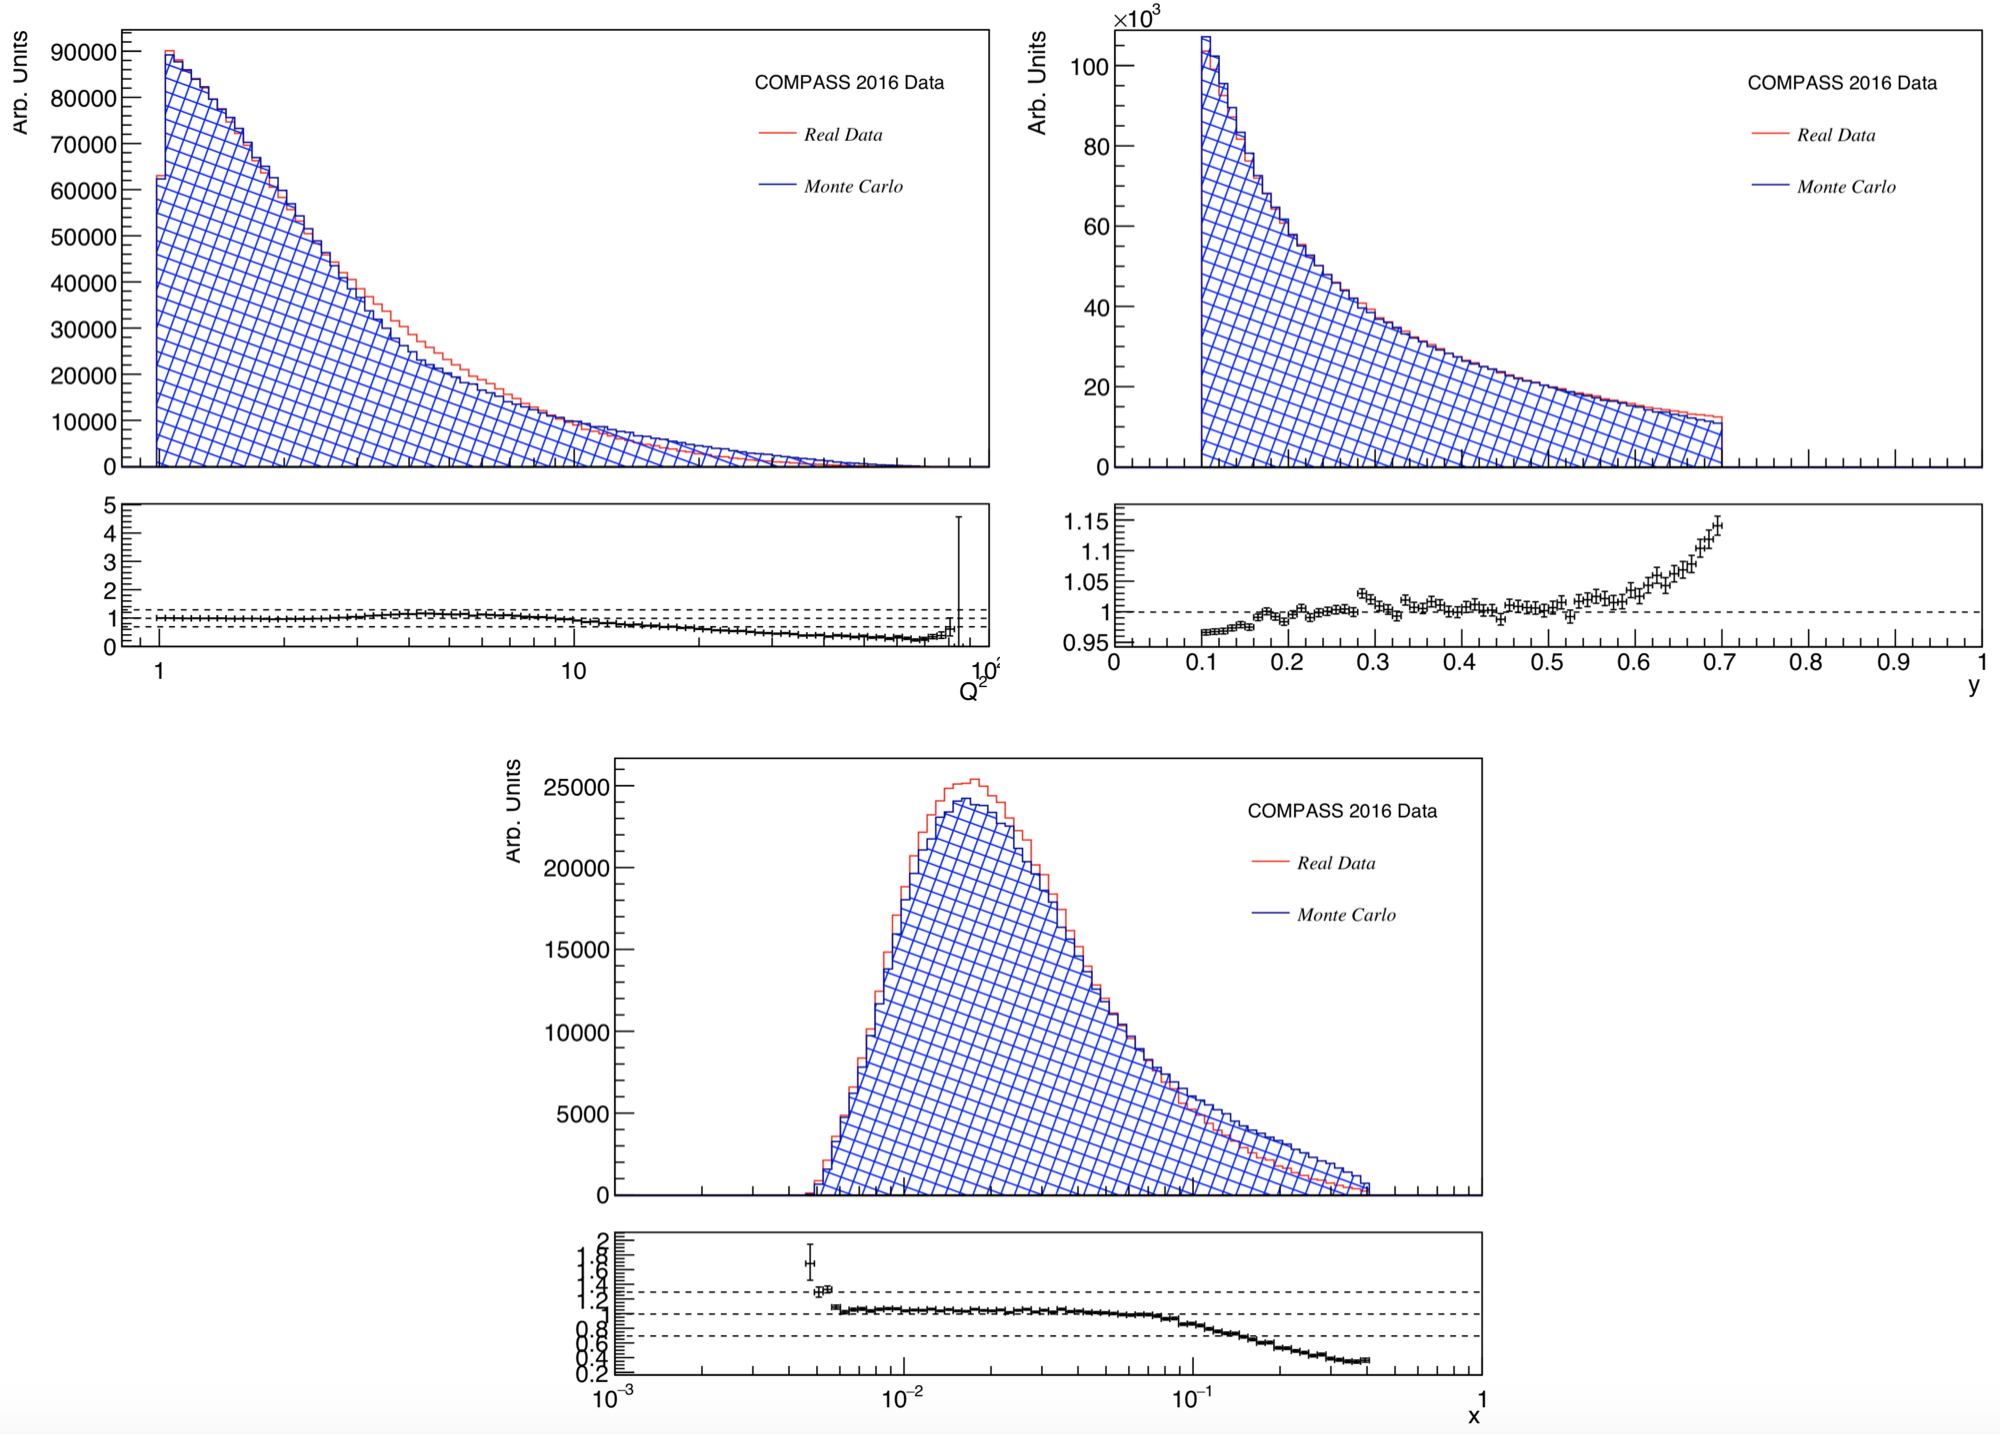
\includegraphics[scale=0.45]{./gfx/DIS_kin.png}
	\caption{Kinematical variables for DIS events ($Q^2$, $y$ and $x$) for Data (red) and Monte-Carlo (blue), as well as the ratio Data/Monte-Carlo.}
	\label{pic:MCDISkin}
\end{figure}

\begin{figure}[!h]
	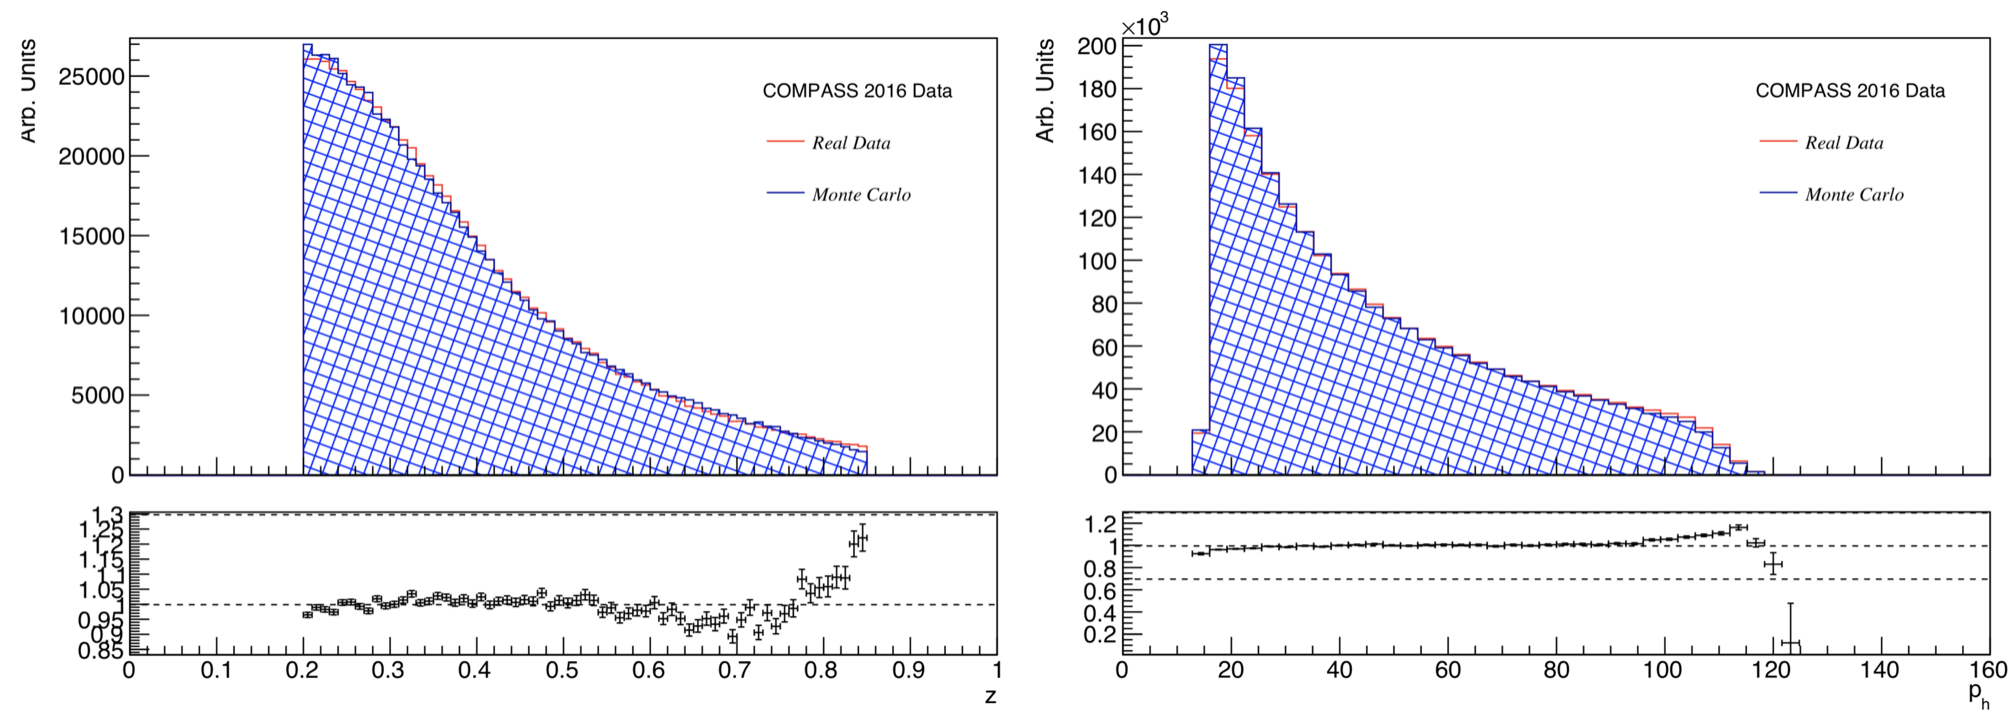
\includegraphics[scale=0.45]{./gfx/SIDIS_kin.png}
	\caption{Kinematical variables for charged hadrons ($z$ and $p_h$) for Data (red) and Monte-Carlo (blue), as well as the ratio Data/Monte-Carlo.}
	\label{pic:MCSIDISkin}
\end{figure}

\subsection{Acceptance calculation}

In the following, $r$ and $g$ refers to 'reconstructed' and 'generated' quantities.

The acceptance is determined as the ratio of reconstructed multiplicities $M^h_r$ over the generated multiplicities $M^h_g$ and is binned in $x$, $y$ and $z$ :

\begin{equation}
  A^h(x,y,z) = \frac{M^h_r(x,y,z)}{M^h_g(x,y,z)}=\frac{N^h_r(x,y,z)/N^{DIS}_r(x,y,z)}{N^h_g(x,y,z)/N^{DIS}_g(x,y,z)}
\end{equation}

where $x_g$, $y_g$ and $z_g$ are the generated kinematic values and $x_r$, $y_r$ and $z_r$ are the reconstructed kinematic values.

The acceptance correction factors $A^h(x,y,z)$ for unidentified hadrons, pions, kaons and protons are shown in Figs. \ref{pic:AccH} to \ref{pic:AccP} for the P07 sample.

\begin{sidewaysfigure}[!]
	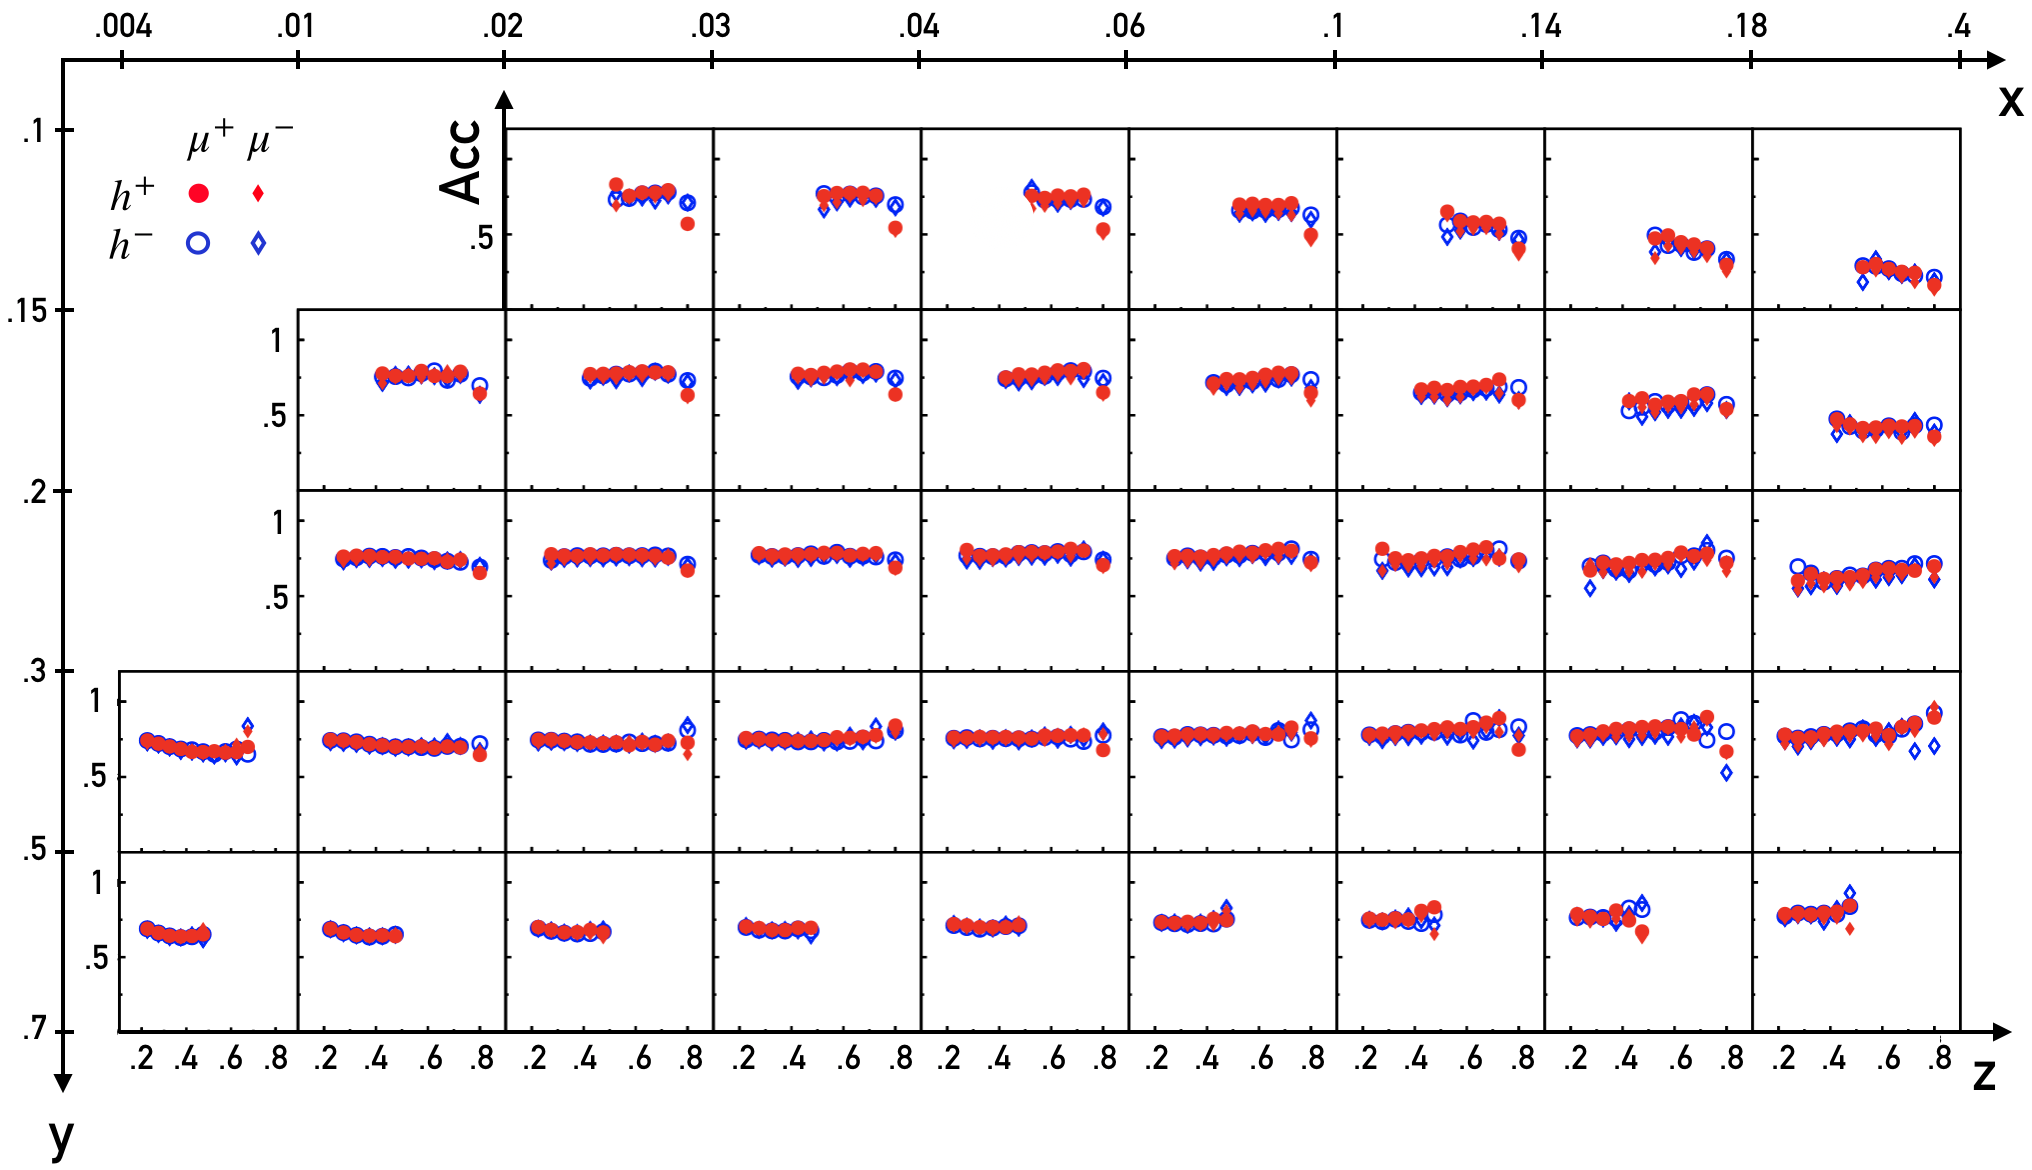
\includegraphics[scale=0.6]{./gfx/AccH.png}
	\caption{Charged hadron acceptance in $x$, $y$ and $z$ bins. The red markers correspond to positive hadrons, blue markers to negative hadrons, circles markers correspond to hadrons obtained with $\mu^+$ beam and diamonds markers to hadrons obtained with $\mu^-$ beam.}
	\label{pic:AccH}
\end{sidewaysfigure}

\begin{sidewaysfigure}[p]
	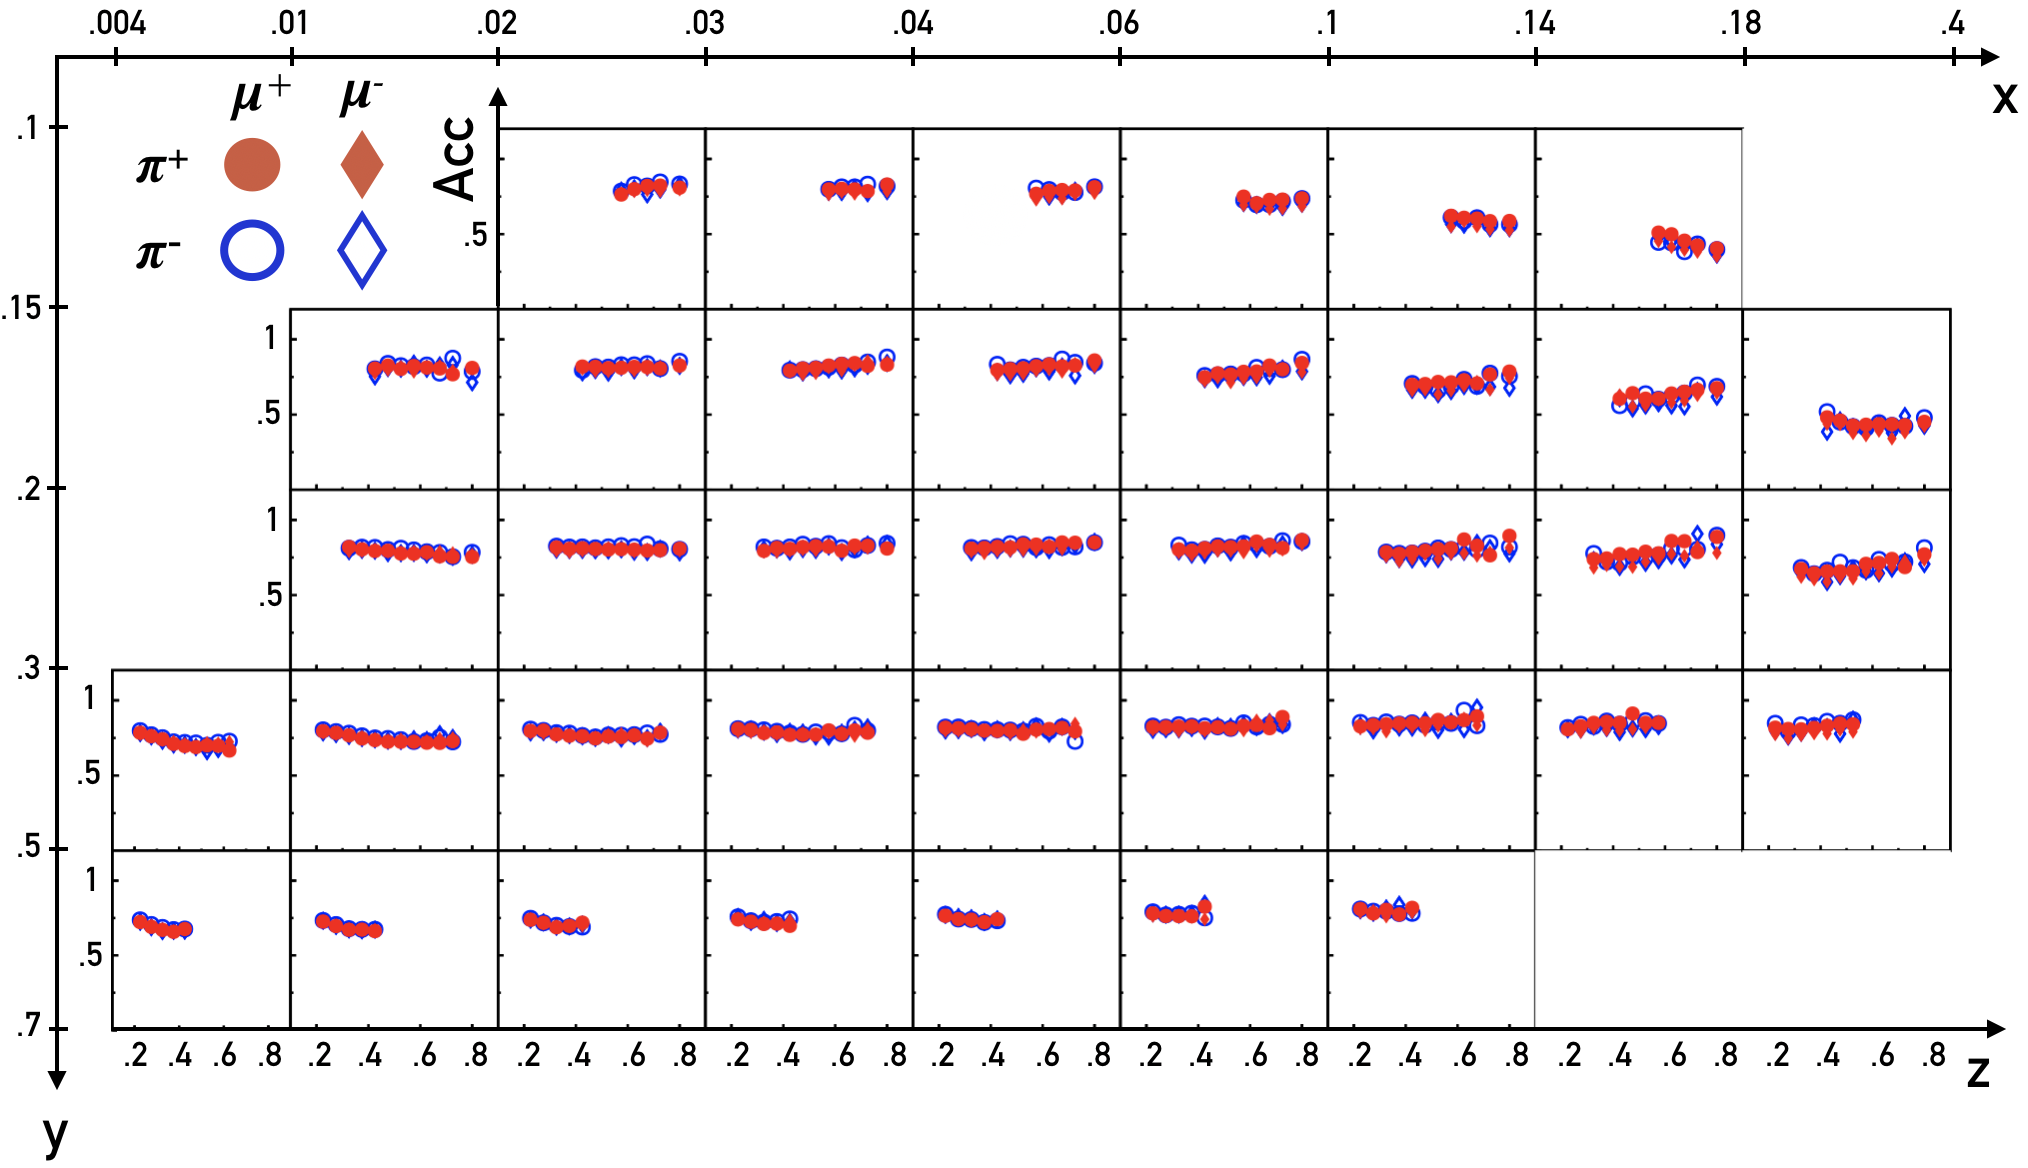
\includegraphics[scale=0.5]{./gfx/AccPi.png}
	\caption{Charged pion acceptance in $x$, $y$ and $z$ bins. The red markers correspond to positive hadrons, blue markers to negative hadrons, circles markers correspond to pions obtained with $\mu^+$ beam and diamonds markers to hadrons obtained with $\mu^-$ beam.}
	\label{pic:AccPi}
\end{sidewaysfigure}

\begin{sidewaysfigure}[p]
	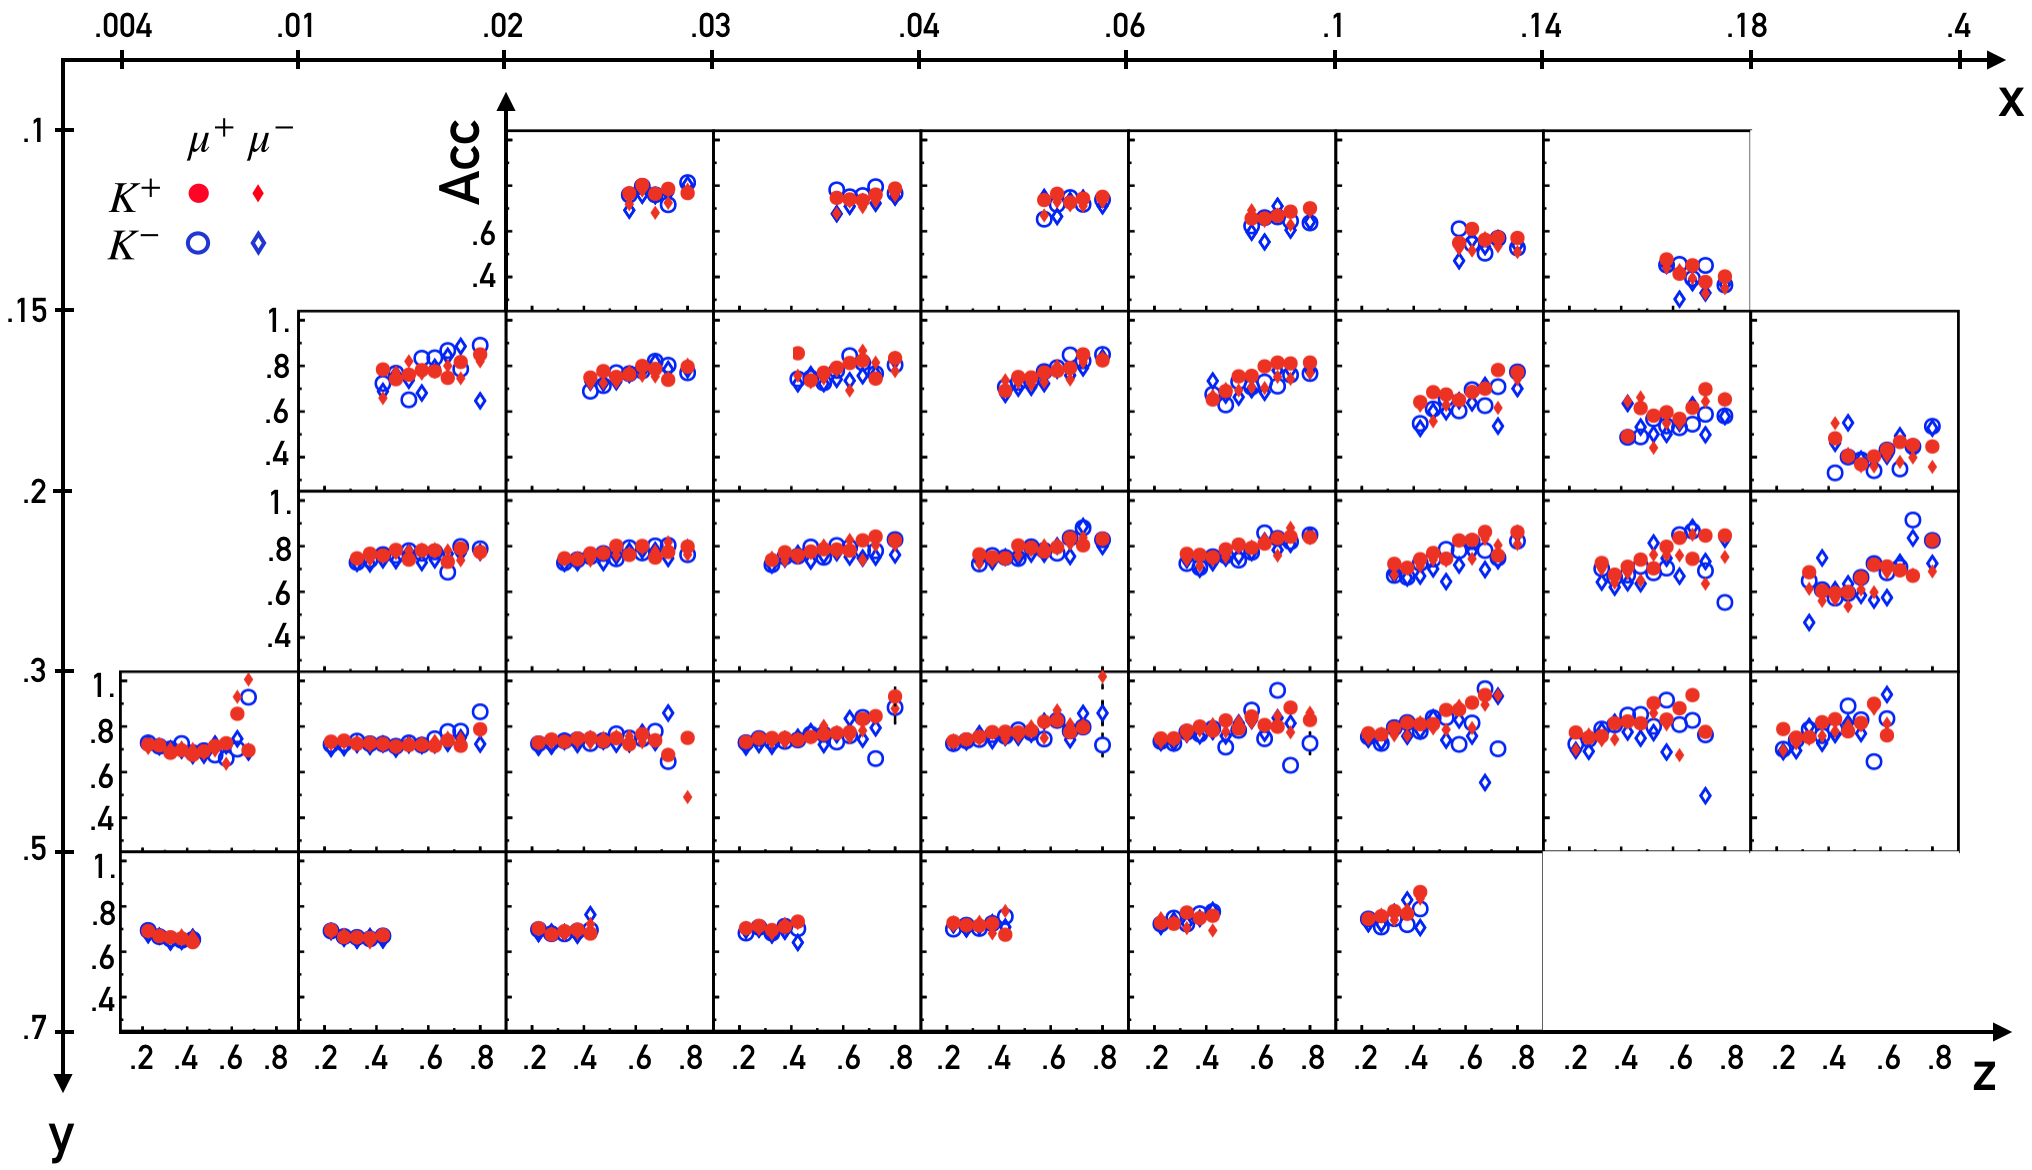
\includegraphics[scale=0.5]{./gfx/AccK.png}
	\caption{Charged kaon acceptance in $x$, $y$ and $z$ bins. The red markers correspond to positive hadrons, blue markers to negative hadrons, circles markers correspond to kaons obtained with $\mu^+$ beam and diamonds markers to hadrons obtained with $\mu^-$ beam.}
	\label{pic:AccK}
\end{sidewaysfigure}

\begin{sidewaysfigure}[p]
	% 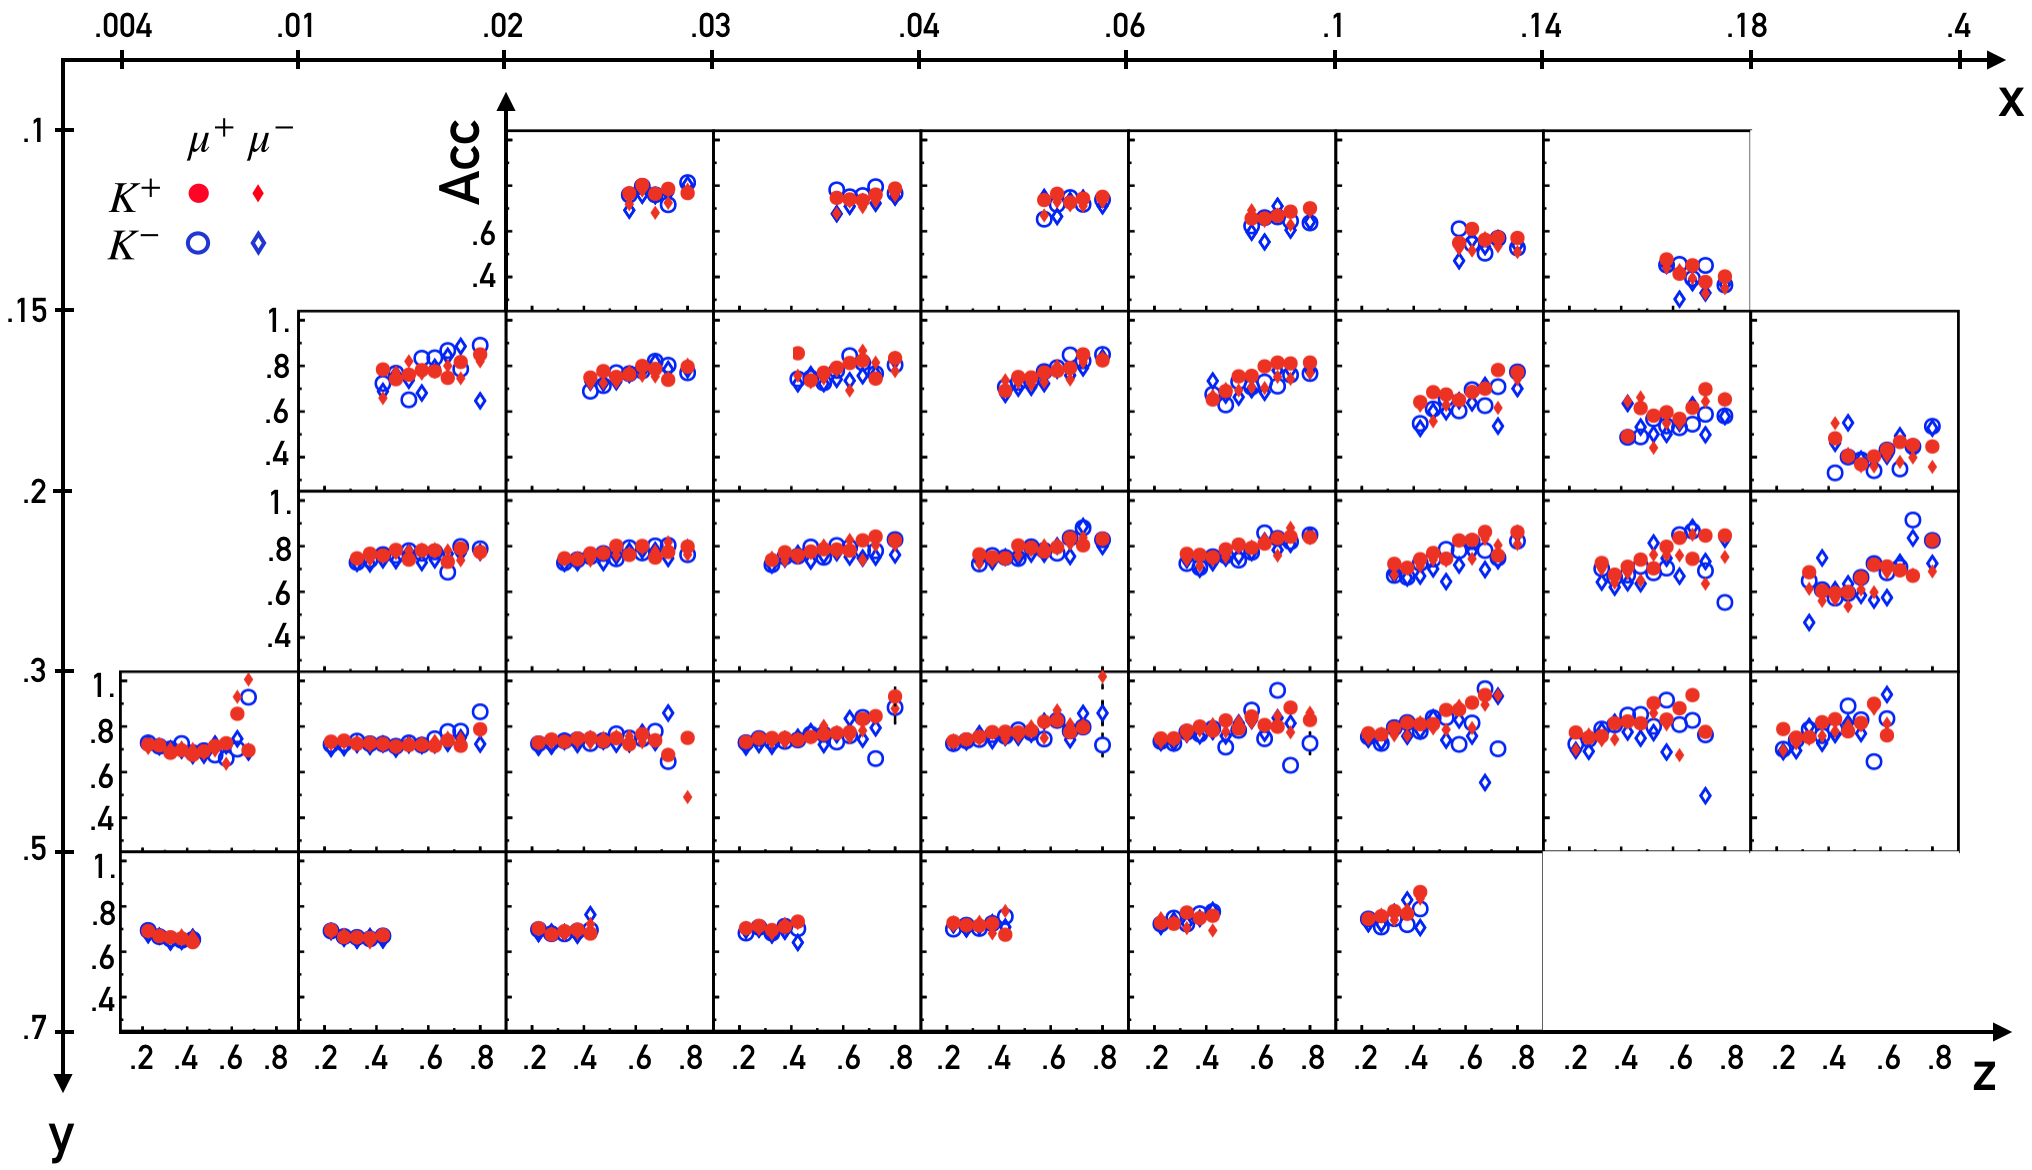
\includegraphics[scale=0.5]{./gfx/AccK.png}
	\caption{Charged proton acceptance in $x$, $y$ and $z$ bins. The red markers correspond to positive hadrons, blue markers to negative hadrons, circles markers correspond to kaons obtained with $\mu^+$ beam and diamonds markers to hadrons obtained with $\mu^-$ beam.}
	\label{pic:AccP}
\end{sidewaysfigure}

In Fig. \ref{pic:AccPer} are compared the acceptance correction factors for the P07 and P09 samples. The discrepancy is only visible on the highest $x$ bins.

\begin{sidewaysfigure}[p]
	% 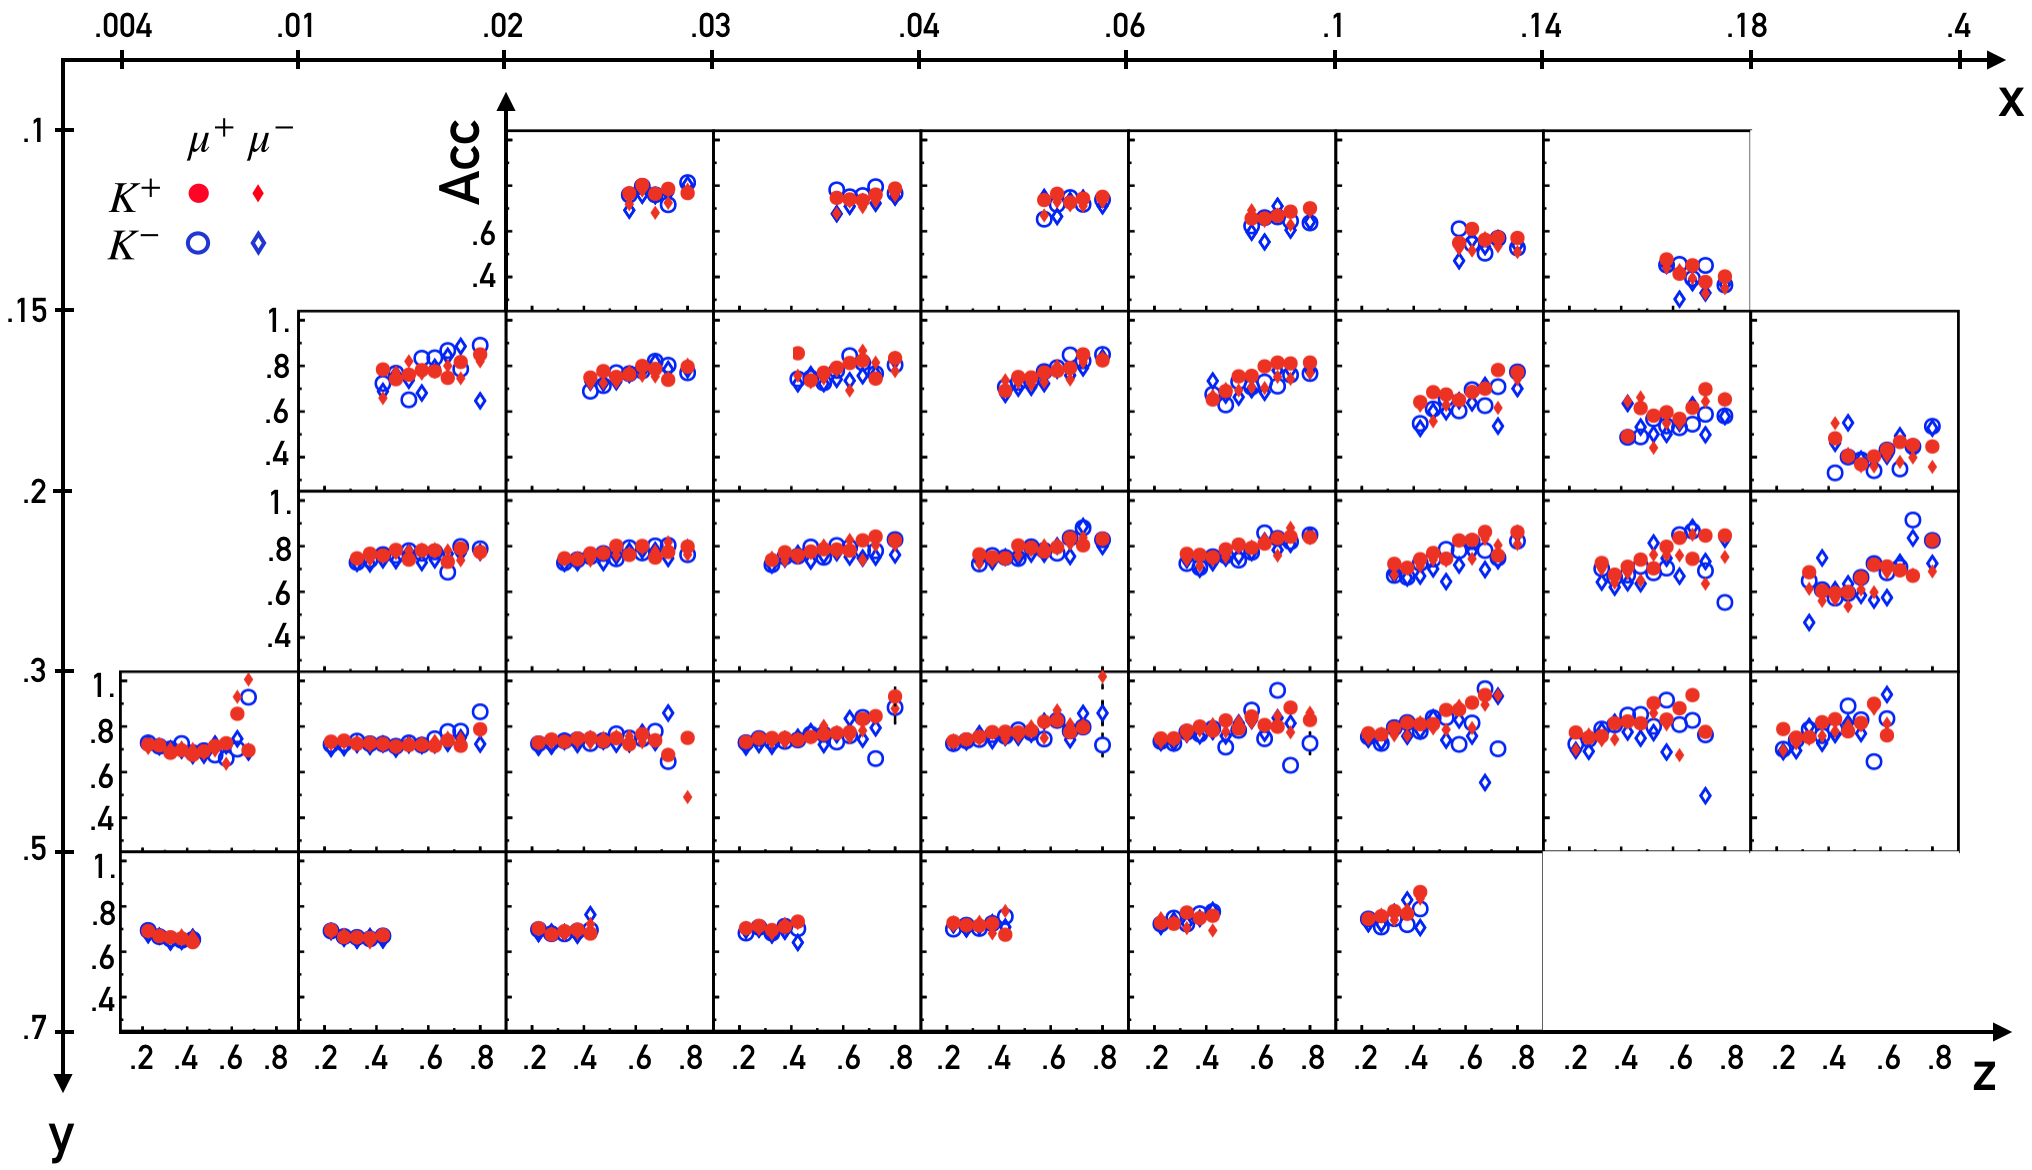
\includegraphics[scale=0.5]{./gfx/AccK.png}
	\caption{-}
	\label{pic:AccPer}
\end{sidewaysfigure}

Used in this fashion, the kinematic bin smearing due to reconstruction limitations is accounted for. A more rigorous bin smearing correction would involve an unfolding procedure but is not done in this analysis.

For this method, the error estimation is difficult to rigorously calculate as the numbers of evaluated hadrons and DIS events, in both the reconstructed and generated case, are not independent. An estimation is made by considering that the hadrons numbers and DIS events are independent of each other. Due to the $z$ kinematic bin migration effects, there exist particles in $N_r$ which are independent from $N_g$. Decomposing $N_r$ into two independent samples namely $N_{r^0}$ which are contained in $N_g$ and $N_{r'}$ which are not, the final acceptance error yields :

\begin{equation}
  \begin{split}
    E^2_{acc} = \left (\frac{G_D}{R_D+R'_{D}}\right )^2\left [\frac{(R_h+A)(G_h-R_h+1)}{(G_h+2)^2(G_D+3)}+\frac{R'_{h}}{G^2_h}+\frac{R'^2_h}{G^3_h}\right ] \\
                + \left (\frac{G_D}{R_D+R'_{D}}\right )^4\left (\frac{R_h+R'_h}{G_h}\right )^2\left [\frac{(R_D+1)(G_D-R_D+1)}{(G_D+2)^2(G_D+3)}+\frac{R'_D}{G^2_D}+\frac{R'^2_D}{G^3_D}\right ]
  \end{split}
\end{equation}

where $G_h$ (resp. $G_D$) are the generated hadrons (resp. DIS events) in a given $x$, $y$, $z$ bin, $R_h$ (resp. $R_D$) the reconstructed hadrons (resp. DIS events) and $R'_h$ (resp. $R'_D$) all other particles (resp. events) that are reconstructed as hadrons (resp. DIS events) in a given $x$, $y$, $z$ bin.

The correction is then applied to the raw multiplcities :

\begin{equation}
  M^h(x,y,z) = \frac{M^h_{raw}(x,y,z)}{A^h(x,y,z)}
\end{equation}

\newpage

\section{Diffractive vector meson correction}

It is usually assumed that hadrons produced in SIDIS originate from lepton-parton scattering. Nevertheless the scattering of a lepton off a nucleon can also result in the diffractive production of vector mesons. These particles decay into lighter mesons that cannot be distinguished from the one resulting from the hadronization of a quark originating from the target nucleon. This implies that fragmentation functions extracted from multiplicities contaminated with diffractive vector mesons would violate universality, as they would be process dependent. However, this is a complex theoretical discussion so the multiplicities both with and without subtracting the diffractive vector meson contribution are calculated as well as the separate correction factors for DIS events and hadrons.

For kaons, the dominant vector meson contribution comes from the diffractive production of $\rho^0$ and $\Phi$ :
\begin{equation}
    \gamma * p \rightarrow \rho^0 p \rightarrow p\pi^+\pi^-
    \gamma * p \rightarrow \Phi p \rightarrow pK^+K^-
\end{equation}

This process is mainly exclusive but in 20\% of cases a diffractive dissociation of the target nucleon occurs. Other channels (excited $\rho$, $\omega$, etc.) are expected to contribute much less and are not taken into account. As pions and kaons stemming from diffractive vector meson decay cannot be separated from the one resulting from SIDIS, the evaluation of their contribution to the multiplicities is based on a Monte Carlo study. Three Monte Carlo samples are produced based on different generators (SIDIS using DJANGOH, diffractive $\Phi$ using HEPGEN++) and the same event reconstruction chain. For the diffractive vector meson samples, both exclusive events and events with diffractive dissociation of the proton are simulated. The $\rho^0$ sample includes nuclear effects (coherent production and nuclear absorption).

The fraction of pions (resp. kaons) resulting from a diffractive $\rho^0$ (resp. $\Phi$) is calculated in the same binning as the raw multiplicities as :

\begin{equation}
  \begin{split}
    f^{\pi}_{\rho^0}(x,y,z) = \frac{N^{\pi}_{HEPGEN++}(x,y,z)}{N^{\pi}_{DJANGOH}(x,y,z)+N^{\pi}_{HEPGEN++}(x,y,z)} \\
    f^K_{\Phi}(x,y,z) = \frac{N^K_{HEPGEN++}(x,y,z)}{N^K_{DJANGOH}(x,y,z)+N^K_{HEPGEN++}(x,y,z)}
  \end{split}
\end{equation}

where $N^{\pi}_{HEPGEN++}$, $N^{\pi}_{DJANGOH}$, $N^K_{HEPGEN++}$ and $N^K_{DJANGOH}$ are the number of kaons reconstructed from the HEPGEN++ and DJANGOH MC samples normalized by the corresponding MC luminosity ($L_{MC}$). The luminosity depends on the event weighting and the process cross-section $\sigma_{int}$ (DIS for DJANGOH event and diffractive vector meson production for HEPGEN++ events). The final weighted number of DIS events and hadrons is summarized in Table \ref{DVM}.

\begin{equation}
  \sum_{events} w_i = L_{MC} \cdot \sigma{int}
\end{equation}

\begin{table}
	\centering
	\begin{tabular}{rccc}
    \hline
     & DJANGOH & $\rho^0$ & $\Phi$ \\
    \hline
    Generated Events & 8.4M & 19.1M & 19.2M  \\
    Weighted Generated Events & 8.4M & 280.2M & 576.9M  \\
		Integrated Cross-Section [pb] & 227010 & 12200 & 2500  \\
		Monte-Carlo Luminosity [pb$^-1$] & 36.8 & 22966.6 & 23075.2  \\
    \hline
		DIS Events [pb] & 3.4M & 96209.4 & 18083.2  \\
		$h^+$ [pb] & 630880 & 25301.9 & 3890.26  \\
		$h^-$ [pb] & 511014 & 25250.4 & 4033.93  \\
		$\pi^+$ [pb] & 453794 & 25257.4 & -  \\
		$\pi^-$ [pb] & 377335 & 25212.3 & -  \\
		$K^+$ [pb] & 102019 & - & 3872.66  \\
		$K^-$ [pb] & 75158 & - & 4015.85 \\
  \end{tabular}
  \caption{Weighted number of DIS events and hadrons for the diffractive vector meson correction. Results cross-checked with A. Moretti.}
  \label{DVM}
\end{table}

The diffractive vector meson events can also lead to a contamination in DIS events. Here, the two channels studied are diffractive $\rho^0$ and $\Phi$ with the fraction of the contamination expressed in Eqs. 13. Contrary to previous Eq. 11, the denominator only includes the DIS events from the DJANGOH generator because the cross-section used to generate the DJANGOH sample takes into account the diffractive contribution.

\begin{sidewaysfigure}[!]
	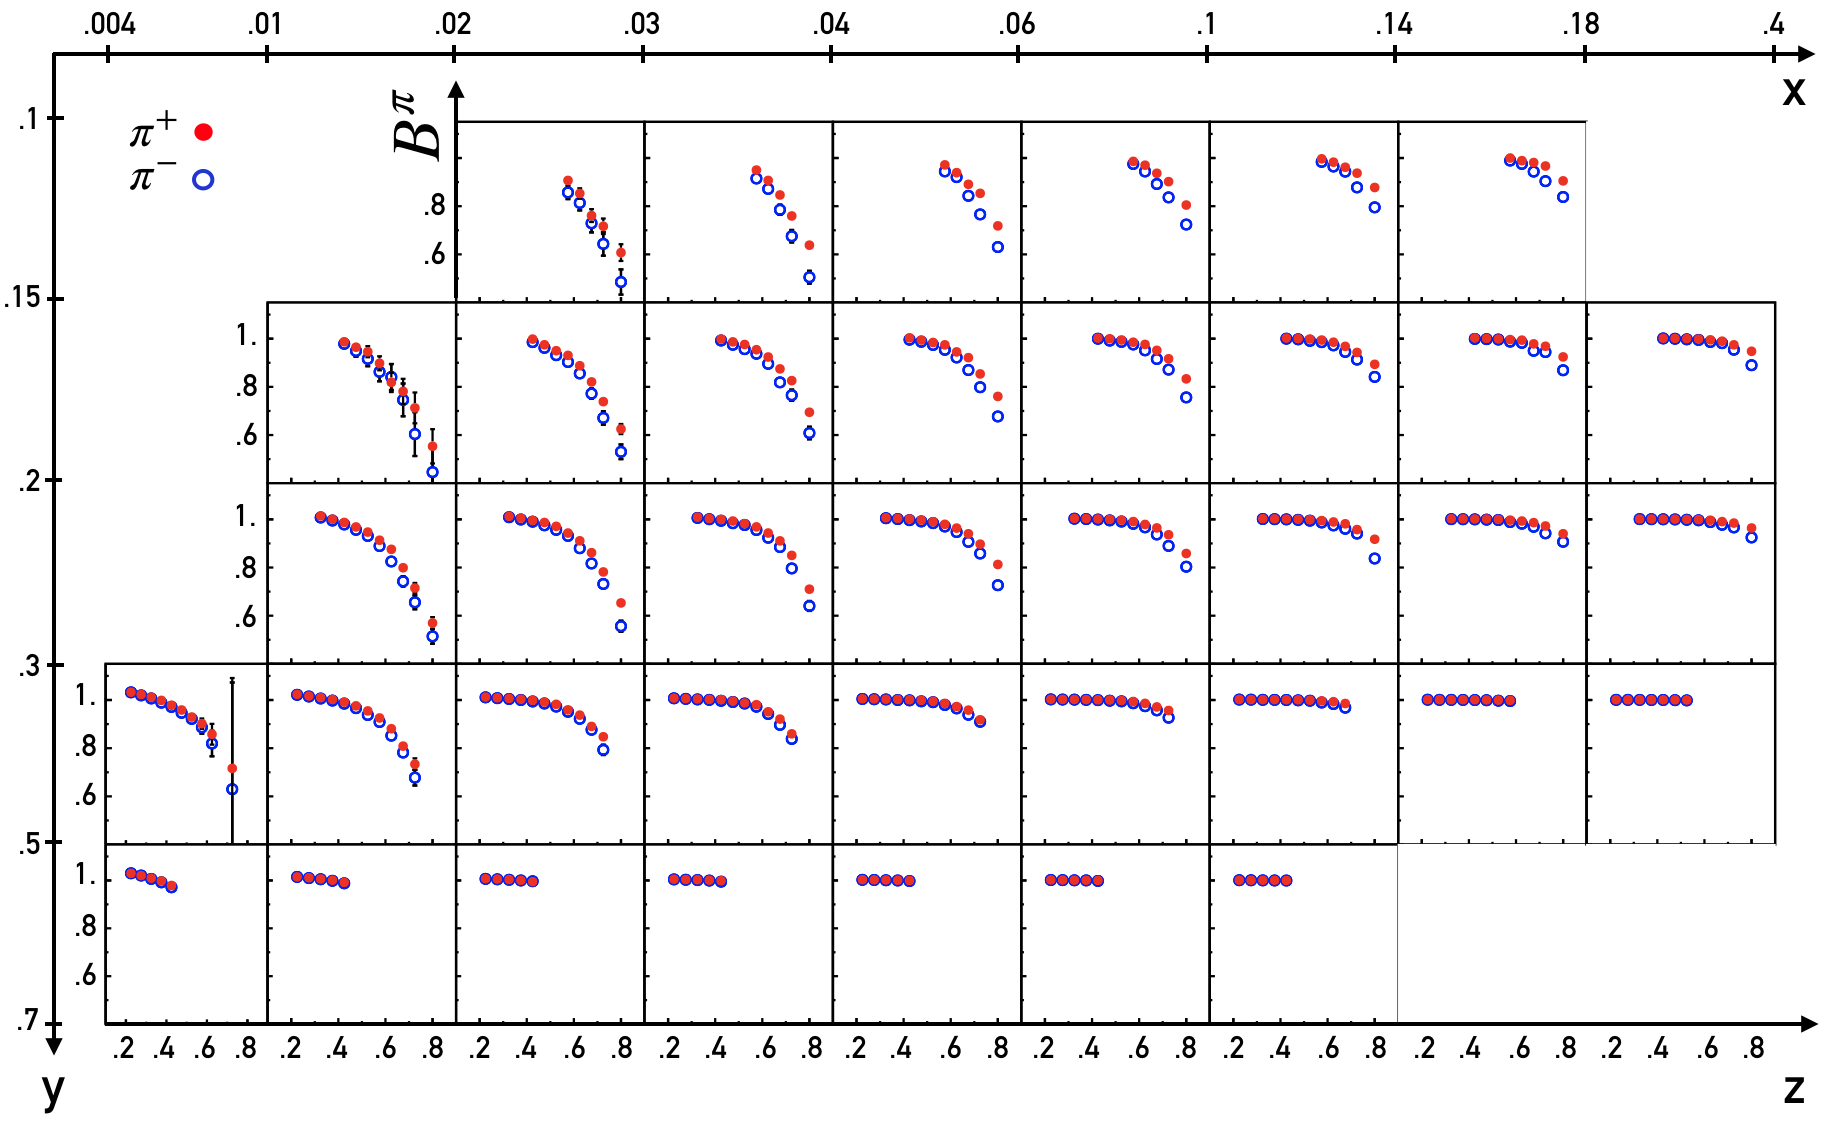
\includegraphics[scale=0.5]{./gfx/DVMpi.png}
	\caption{Correction factor $B^{\pi}$ for diffractive vector meson contamination as a function of $z$ for ($x$,$y$) bins. The red markers correspond to positive pions and blue markers for negative pions.}
	\label{DVMpi}
\end{sidewaysfigure}

\begin{sidewaysfigure}[!]
	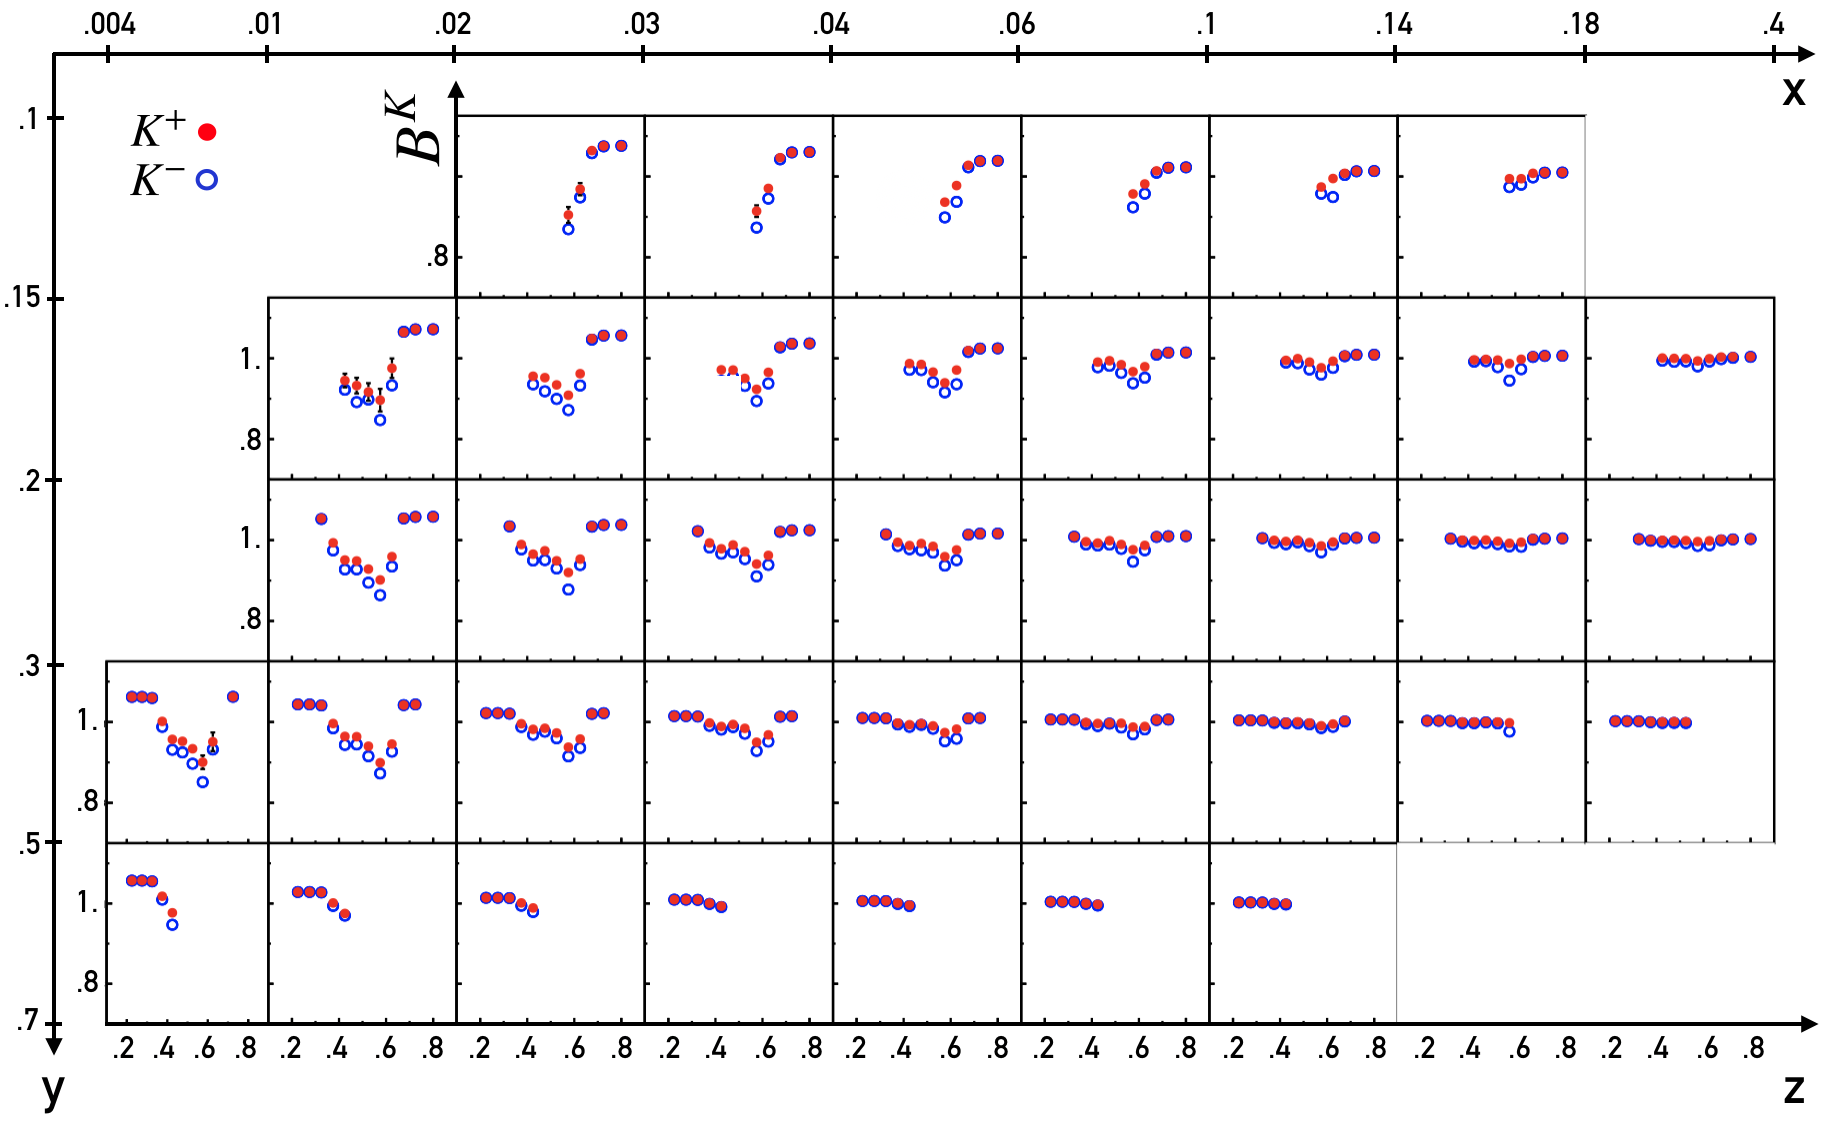
\includegraphics[scale=0.5]{./gfx/DVMK.png}
	\caption{Correction factor $B^{K}$ for diffractive vector meson contamination as a function of $z$ for ($x$,$y$) bins. The red markers correspond to positive kaons and blue markers for negative kaons.}
	\label{DVMK}
\end{sidewaysfigure}

\begin{equation}
  \begin{split}
    f^{\rho^0}_{DIS}(x,y,z) = \frac{N^{DIS}_{\rho^0,HEPGEN++}(x,y,z)}{N^{DIS}_{DJANGOH}(x,y,z)+N^{DIS}_{\rho^0,HEPGEN++}(x,y,z)+N^{DIS}_{\Phi,HEPGEN++}(x,y,z)} \\
    f^{\Phi}_{DIS}(x,y,z) = \frac{N^{DIS}_{\Phi,HEPGEN++}(x,y,z)}{N^{DIS}_{DJANGOH}(x,y,z)+N^{DIS}_{\rho^0,HEPGEN++}(x,y,z)+N^{DIS}_{\Phi,HEPGEN++}(x,y,z)}
  \end{split}
\end{equation}

The total contribution from the diffractive vector-meson contribution ($f^{VM}_{DIS}$) to the DIS sample is the sum of the $f^{\rho^0}_{DIS}$ and $f^{\Phi}_{DIS}$. The final correction reads as follows :

\begin{equation}
  \begin{split}
  B^h(x,y,z) = \frac{ \frac{N^{\pi}(x,y,z)}{N^h(x,y,z)}\left (1-f^{\pi}_{\rho^0}(x,y,z)\right )
                   + \frac{N^K(x,y,z)}{N^h(x,y,z)}\left (1-f^{K}_{\Phi}(x,y,z)\right ) + \frac{N^p(x,y,z)}{N^h(x,y,z)} }{1-f^{VM}_{DIS}(x,y,z)} \\
  B^{\pi}(x,y,z) = \frac{1-f^{\pi}_{\rho^0}(x,y,z)}{1-f^{VM}_{DIS}(x,y,z)} \\
  B^K(x,y,z) = \frac{1-f^{K}_{\Phi}(x,y,z)}{1-f^{VM}_{DIS}(x,y,z)}
  \end{split}
\end{equation}

The correction for pions has the strongest impact at high $z$ ($z>0.5$) and low $x$ ($x<0.02$) where it can reach 50\%, while the correction for kaons has the strongest impact at middle $z$ ($0.4<z<0.6$) and low $x$ ($x<0.02$) where it can reach 20\%.

\section{Radiative corrections}

The experimental multiplicities are affected by QED radiative effects, which introduces a systematic bias of the measured kinematics with respect to the true kinematics. The most important contributions at first order are the initial and final state radiation of a real photon by the incoming or outgoing lepton. The correction factor used to take into account these phenomena is the radiative correction factor defined as :

\begin{equation}
	\eta(x,y,z) = \frac{d^2 M_{1\gamma}/dxdydz}{d^2 M_{measured}/dxdydz}
\end{equation}

where $M_{1\gamma}$ denotes multiplicities obtained using the cross-section in the one photon exchange approximation and $M_{measured}$ denotes multiplicities obtained using the measured cross-section which includes radiative effects. The bias on the $\mu$ kinematics upon real photon emission affects in turn the reconstruction of the hadron energy fraction $z$. This effect is now taken into account thanks to DJANGOH. In this analysis, the multiplicities are directly corrected. Fig.\ref{fig:hadz_ratio} in Chapter \ref{ch:RC}, Section \ref{sec:RCFMult} shows the effect of the correction.

\section{Electron contamination}

The pion (and thus hadron) sample is contaminated by electrons and positrons. With the DJANGOH event generator, we are able to describe almost correctly the electron production from radiative photons : in Fig.\ref{electroprod} one can see that the discrepancy of electroproduction along $\Phi$ in the hadron production plane differ by 10\% at low $\Phi$. Given the overall small size of the correction it is reasonable to use the MC sample at momenta where the electron identification cannot be provided by the RICH detector. The fraction of electrons in the hadron and pion samples obtained in the range 12 $< p_h <$ 40 GeV in the MC sample is shown in Figs. \ref{pic:ehad} and \ref{pic:epi}. This contamination goes from 8\% at low $z$ to 1\% at high $z$. The correction is taken into account in the acceptance correction, taking in the electrons in the reconstructed sample (as in data) and not in the generated one. In a discussion afterwards on the multiplicity sum of pions and hadrons, it might be that we are correcting only partially for this contamination.

\begin{figure}[!]
	% 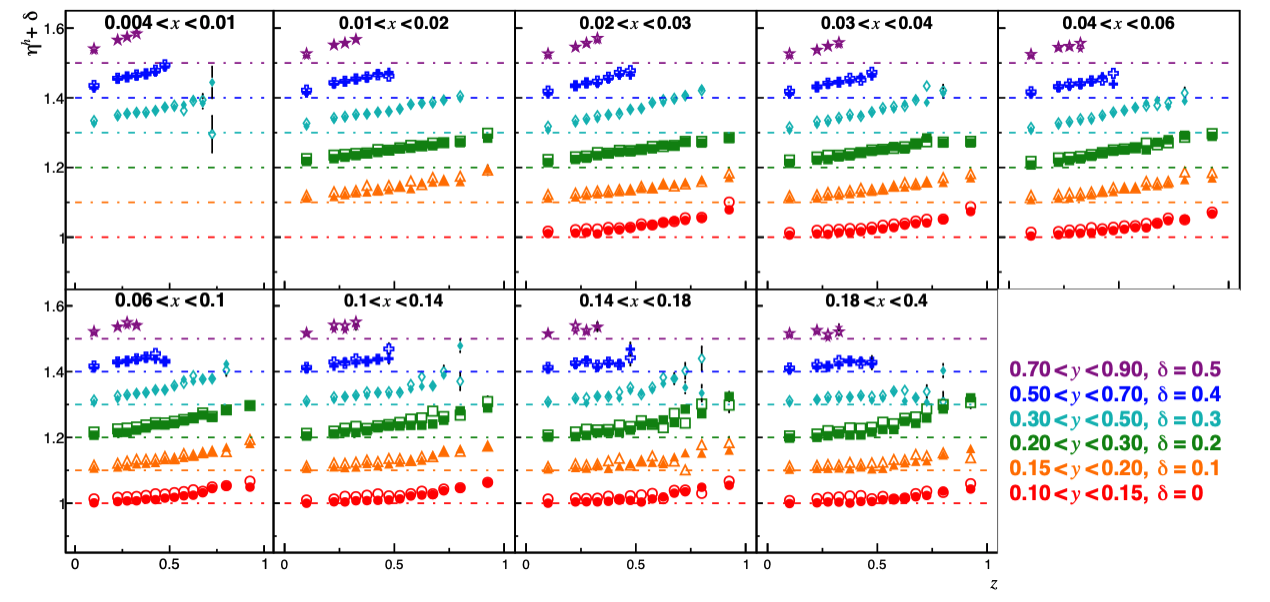
\includegraphics[scale=0.5]{./gfx/RadCor.png}
	\caption{Electron corrections (TBD)}
	\label{pic:ehad}
\end{figure}

\begin{figure}[!]
	% 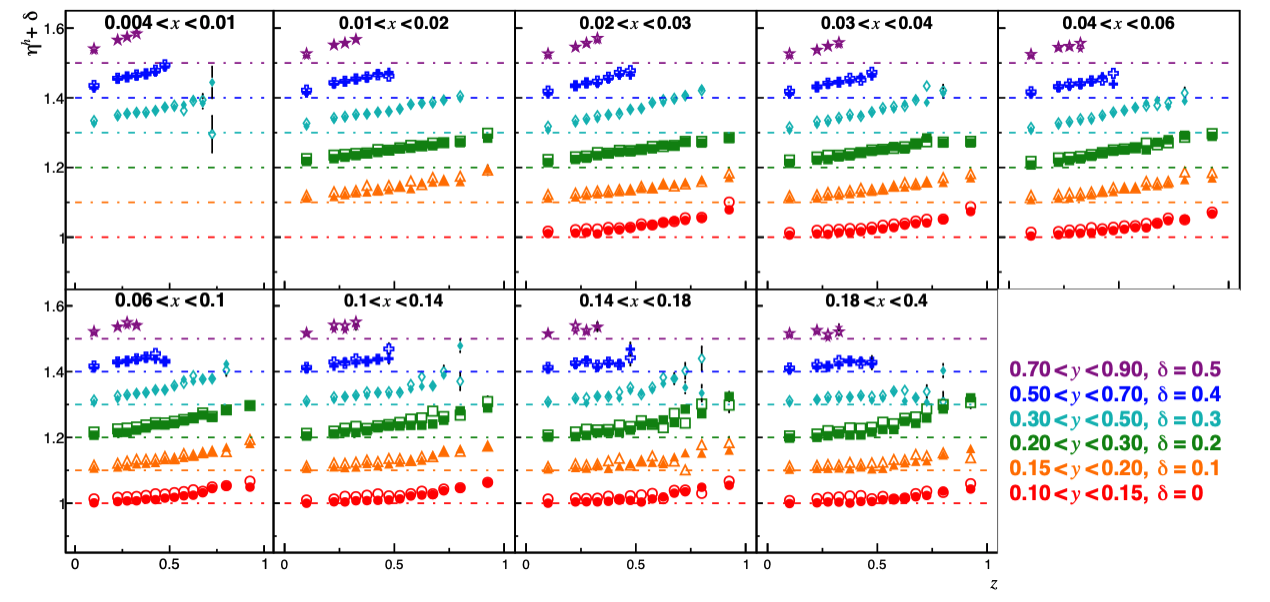
\includegraphics[scale=0.5]{./gfx/RadCor.png}
	\caption{Electron corrections (TBD)}
	\label{pic:epi}
\end{figure}
